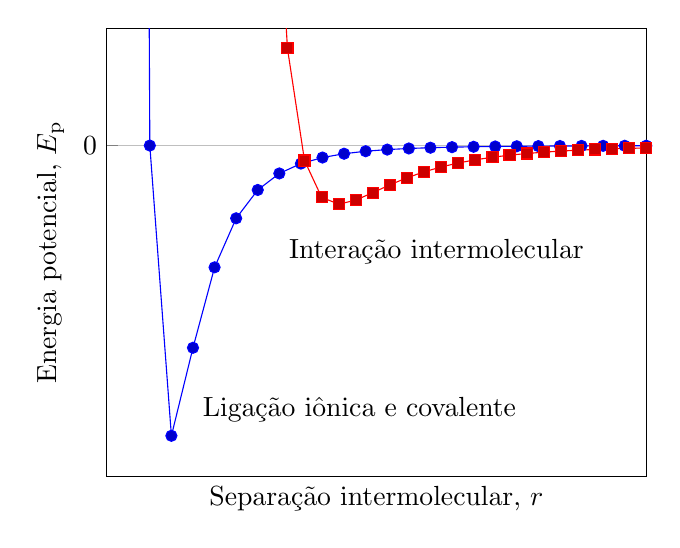
\begin{tikzpicture}
    \begin{axis}
    [
        grid = major,
        ylabel = {Energia potencial, $E_\mathrm{p}$},
        xlabel = {Separação intermolecular, $r$},
        xmin = 0.5, xmax = 3,
        ymax = 2,
        xtick=\empty, ytick=0,
    ]
    \addplot+[domain=0.6:3]
        {
            4 * 5 * ((0.7/x)^(12) - (0.7/x)^6)
        };
    \addplot+[domain=1.1:3]
        {
            4 * 1 * ((1.4/x)^(12) - (1.4/x)^6)
        };
    \node [anchor=west] at (axis cs:0.9,-4.5) {Ligação iônica e covalente};
    \node [anchor=west] at (axis cs:1.3,-1.8) {Interação intermolecular};
\end{axis}
\end{tikzpicture}
